\documentclass[12pt]{article}

\title{Using idiolects to improve word prediction}
\author{Wessel Stoop}

\usepackage{covington}
\usepackage{graphicx}
\usepackage{natbib}
\usepackage{float}

\renewcommand{\familydefault}{\sfdefault}

\let\stdsection\section
\renewcommand\section{\newpage\stdsection}

\begin{document}

\begin{table}[b]
\begin{tabular}{ll}
\textbf{Master's thesis}&\\
Name&Wessel Stoop\\
Student numbers&s0808709 (Nijmegen), u1249664 (Tilburg)\\
Supervisor&Antal van den Bosch\\
Period&Spring 2013\\
\end{tabular}
\end{table}

\maketitle

\begin{figure}
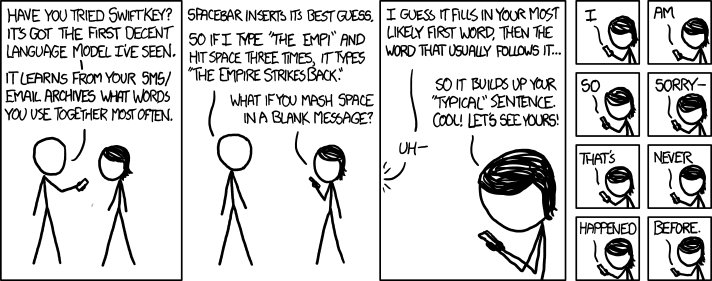
\includegraphics[scale=0.5]{swiftkey}
\end{figure}

\clearpage

\tableofcontents

\section{Summary}

\section{Introduction}

\subsection{Word prediction}

%Eerst algemeen
%Daarna laatste ontdekkingen

\subsection{Idiolects}




%Uitleg: twee delen. Dat zijn de volgende twee sections






\section{The algorithm: Soothsayer}

\subsection{Introduction}

\subsubsection{Soothsayer}
The goal of this chapter is to build the best word prediction algorithm possible, from the ground up. We will start with a very basic application that uses word uniqueness thresholds to predict the word the user is keying in, and add more components and smaller improvements step by step. I have given the resulting system the working title \emph{Soothsayer}, for ease of reference.

An important thing to note is that Soothsayer works with independent modules. A module can be seen as a function that takes some input (for example, the letters of the word the user is currently keying in), uses a language model to generate:

\begin{enumerate}
\item The most likely prediction
\item The second most likely prediction
\item The third most likely prediction
\item In case of a context-sensitive module, how many other predictions the model provided
\end{enumerate}

Modules can be either context-insensitive or context-sensitive, as will be explained in much detail in section \ref{ci} and section \ref{cs} respectively, and use one language model. In a set-up with two language models (which is the main set-up used in chapter \ref{model}), we thus have four possible modules:

\begin{enumerate}
\item Model 1, context-sensitive
\item Model 1, context-insensitive
\item Model 2, context-sensitive
\item Model 2, context-insensitive
\end{enumerate}

Modules can be concatenated in such a way that a second module takes over once the first modules no longer has predictions, a third module takes over once the second one no longer has predictions, etcetera. This makes it possible to use multiple prediction techniques \emph{and} multiple language models in one prediction system.

\subsubsection{Evaluation}
In this chapter, I will propose an addition to Soothsayer and then measure to what extent it improves the number of keystrokes saved several times. But how does one measure how many keystrokes are saved exactly? In other words, what is the best way to evaluate a word prediction system?

%Lit

%CKS SKKS

A thing to notice is that both measures reflect the percentage of keystrokes saved in an ideal situation; that is, when the user accepted a correct prediction immediately once it is available. As will be discussed further in section \ref{early}, this is not necessarily the case. 

%wordt dat echt discussed?

\subsubsection{What Soothsayer is not}
There are many possible approaches to take when building an autocompletion system. Because it would take too much time to try all of these approaches (and all combinations of them), I had to decide. Therefore, before I explain and defend the workings of Soothsayer, I therefore would like to list these decisions, so the reader has a rough idea of what is coming. 

\begin{itemize}
\item Soothsayer does not use hand-made rules and is fully language independent.
%blabla, parsers, voorbeeld
As a result of this, Soothsayer is fully language independent: if it is trained on Dutch data, is will predict Dutch words, if it is trained on Swahili, it will predict Swahili words. In fact, the context-sensitive modules will give correct predictions even with mixed training data.
\item Soothsayer is not designed for mobile phones.

%T9
\item Soothsayer only predicts one word at a time.
\end{itemize}

%Uitleggen

\subsection{Context-insensitive modules} \label{ci}

Context-insensitive modules only use information of the word the users is currently keying in. In sentence \ref{only_c}, for example, only the c will be used for prediction. 

\begin{examples}
\item I ate too much c \label{only_c}
\end{examples}

This means that a prediction like \emph{communication} is fully possible, despite the context, just because \emph{communication} starts with a c. This also means that at the beginning of a each new word no prediction will be available, because the module has no material to work with.

Desprite these limitations, context-insensitive modules can already save a lot of keystrokes, because the first few letters of a word impose enormous limitations on what letters can possibly follow.

\begin{examples}
\item This is good communic \label{communic}
\end{examples}

In sentence \ref{communic}, we already know from \emph{communic} that \emph{ation} or \emph{ative} will follow, simply because these are the only two words that start with \emph{communic}. The first iteration of the context-insensitive module I will propose will be based on this idea: at a certain point in a word, other words are no longer an option. This point is called the \emph{uniqueness threshold}.

\subsubsection{Using uniqueness threshold}

\subsubsection{Using word frequencies}

\subsection{Context-sensitive modules} \label{cs}

\subsubsection{Word prediction as a classification task}

\subsubsection{Nearest neighbour classification}

\subsection{Other decisions}

\subsubsection{Attenuation}

\subsubsection{Punctuation as acceptance key}

\subsubsection{Early prediction switching ???} \label{early}





\section{The model: idiolects} \label{model}

\subsection{A simple experiment}

\subsection{Using Twitter for idiolects}

\subsubsection{Collecting the data}

\subsubsection{Limitations of Twitter data}

\subsection{Language input and networks}

\section{Conclusion}


\section*{Acknowledgements/dankwoord}
% Eenzaam, 'gevecht tussen man en computer'. Bedank Jacintha, Hanna, Iris, Kobie, Ali en Florian.
% Véronique onderwerp, en Lieke voor idiolect ipv ideolect.
% Maarten, Florian en Bouke voor de vele dingen programmeren.
% Antal: mails. Tegelijkertijd waren we met nog veel andere dingen bezig.
% Is ook afsluiting van mijn studententijd. Helen, als tutor en zo ongeveer driekwart van mijn cursussen. G&C
% Hilde: laat Soothsayer spreken

%TODO
% Ergens 'damn you autocompletion' noemen

\end{document}
